\section{Beispiele}
\subsection{Implementierung eines Zustandsautomaten}
Zwei Beispiele zeigen die Verwendung von Intervall-Events bei der
Implementierung von Zustandsautomaten. Zustandsautomaten k"onnen hervoragend
durch die Verwendung von IntervallEvents implementiert werden, da
Zustandsautomaten immer vom Zustand abh"anige Reaktionen auf Events zeigen.

Zur Implementierung kann jeder Zustand des Automaten als ein Intervall
abgebildet werden. Nun kann man Entry-Actions als before-Event an ein Intervall
und Exit-Actions als ein after-Event an das Intervall binden. Transition-Actions
k"onnen wahlweise an das Before- oder das After-Event gebunden werden.
Self-Transitions werden als Vereinigung zwischen dem Intervall-Event und dem
ausl"osenden Event der Self-Transition abgebildet. 

Durch diese Vorgehensweise ergibt sich eine bessere Wartbarkeit des
Quellcodes, da das Programmverhalten nicht mehr imperativ durch If-Statements
oder das Statemachine-Pattern beschrieben wird. Viel mehr wird das
Programmverhalten deklarativ durch Intevall-Events spezifiziert.

Im Rahme dieser Arbeit wurden zwei Zustandsautomaten implementiert. Bei dem
ersten Zustandsautomaten handelt es sich um das vereinfachte Verhalten eines
Filetransfer-Servers dessen Verbindungen offen oder geschlossen sein k"onnen. Der
resultierende Zustandsautomat ist in Abb. \ref{filetransfer_behaviour} zu sehen.

%\usepackage{graphics} is needed for \includegraphics
\begin{figure}[htp]
\begin{center}
  \includegraphics[width=0.15\textwidth]{graphics/tcp_stm.dot.eps}
  \caption{Verhalten einer Filetransfer-Verbindung}
  \label{filetransfer_behaviour}
\end{center}
\end{figure}

\subsubsection{SimpleWebshop-Verhalten}

%\usepackage{graphics} is needed for \includegraphics
\begin{figure}[htp]
\begin{center}
  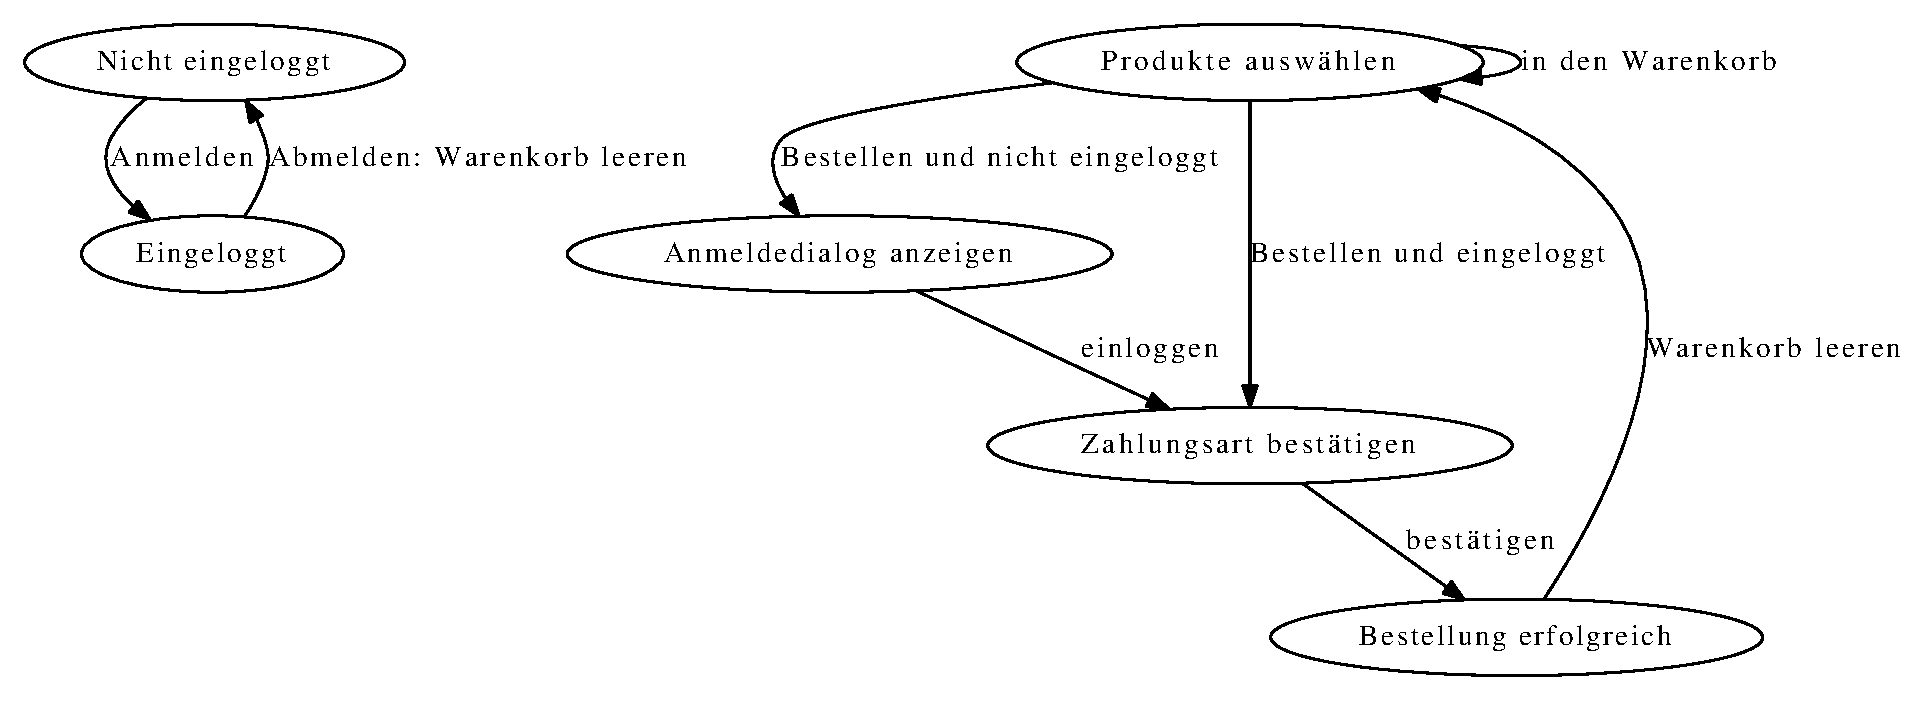
\includegraphics[width=0.6\textwidth]{graphics/webshop.dot.eps}
  \caption{Bestellvorgang in einem Web-Shop}
  \label{webshop_behaviour}
\end{center}
\end{figure}

\subsection{Implementierung einer FileTransfer-Komponente}
Mit File-Sharing-Programmen können Benutzer über ein Computernetzwerk
Dateien austauschen. Wenn ein Benutzer eine Dateiübertragung anfordert, dann
fordert das File-Sharing-Programm von unterschiedlichen Hosts Teile der Datei
an. Die Hosts anworten dann mit den angeforderten Dateiteilen. Daher existiert
in den meisten File-Sharing-Programmen eine Komponente zum Steuern der
Dateiübertragungen. Diese Komponente verwaltet die bereits empfangenen
Dateiteile und kümmert sich darum, noch fehlende Tokens nachzufordern.

Bei der Implementierung einer solchen Komponente bietet sich die Verwendung von
Intervall-Events an. Das Verhalten der FileTransfer-Komponente kann fast
vollständig deklarativ erfolgen. 

\subsection{Implementierung von Ping-Pong}
Als größeres Beispiel wurde im Rahmen des Praktikums das Spiel
Ping-Pong implementiert. In diesem Spiel gibt es ein abgegrenztes Spielfeld mit
Wänden. Im Spielfeld befindet sich ein Ball der sich bewegt. Am Spiel teil
nehmen zwei Spieler die jeweils einen eindimensional beweglichen Schläger haben.
Der Schläger befindet sich vor dem Tor des Spielers. Ziel des Spiels ist es, den
Ball nicht in das eigene Tor zu lassen. Als kleine Erweiterung erscheinen auf
der Spielfläche Geschenke die das Spielverhalten abändern. Die Spielfläche des
Spiels ist in Abb. \ref{ping_pong} zu sehen.

\begin{figure}[htp]
\begin{center}
  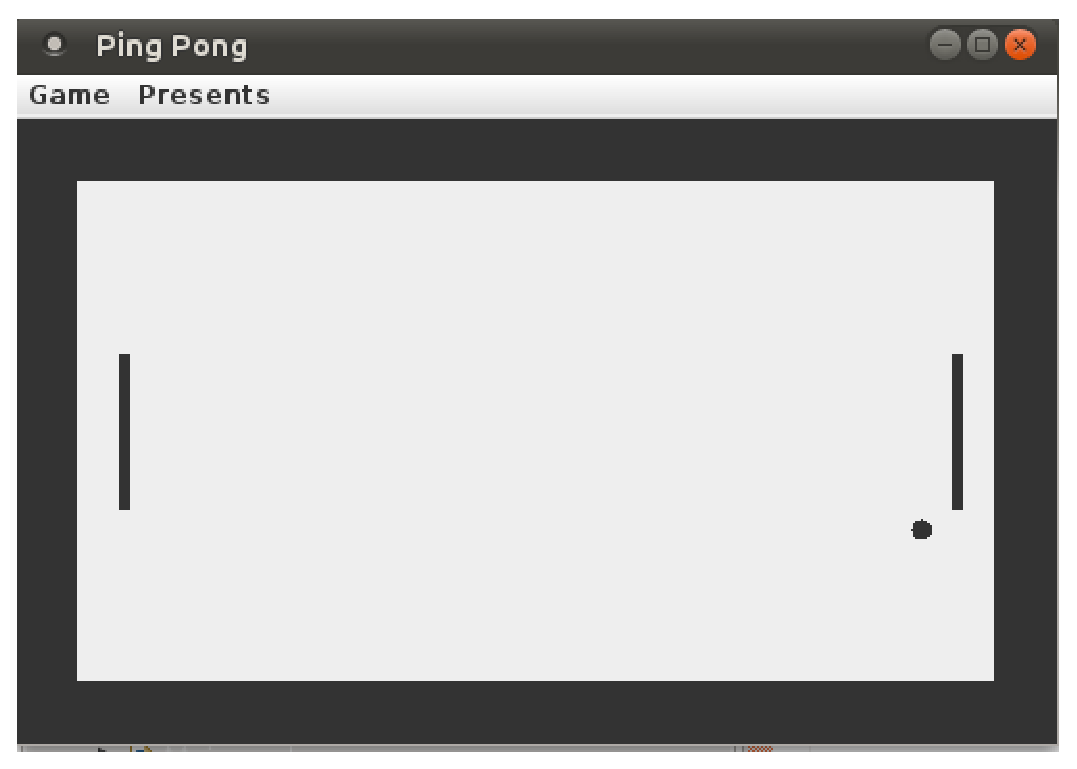
\includegraphics[width=0.6\textwidth]{graphics/pingpong.eps}
  \caption{Ping-Pong}
  \label{ping_pong}
\end{center}
\end{figure}

Das Spielmodell beinhaltet die Wände, den Ball, die Schläger, die Tore und
eventuell Geschenke. Jedes Objekt auf dem Spielfeld hat eine Position und eine
Geschwindigkeit. Allerdings wurde bei der Implementierung des Spiels von der
Klassischen Herangehensweise abgewichen. Klassischerweise besteht ein Spiel aus
einer Spielschleife in der die folgenden Aktionen immer wieder ausgeführt
werden:
\begin{itemize}
  \item Abfragen der Benutzereingaben
  \item Berechnung der Änderungen im Spiel-Modell. Also die Positionsänderung
  des Balls und der Schläger.
  \item Rendern des Spielmodells zu einer Grafik
  \item Warten bis die nächste Iteration notwendig wird. Ohne diese Wartezeit
  hätte man möglicherweise eine zu hohe Frame-Rate.
\end{itemize}


Diese Ansatz ist allerdings nicht Event-Orientiert und wurde daher im Beispiel
nicht verwendet. Stattdesen wird im Beispiel ein Timer verwendet, der alle 50ms
eine Positionsänderung der Objekte und und das Neuzeichnen der Spielfläche auslöst.
Solange ein Spieler eine Bewegen-Taste drückt ist ein Intervall-Event aktiv das
die Geschwindigkeit des Schlägers ändert\footnote{Dies ist übrigens ein
eleganter Workaround für einen Bug in der Java AWT. Mehr Informationen zum
diesem Fehler finden sich unter
bugs.sun.com/view\_bug.do?bug \_id=4153069}.

Weiterhin werden Intervall-Events eingesetzt, um das Zeitmodell des Spiels
abzubilden. Geschenke beispielsweise sollen nur für eine definierte Zeit
vorhanden sein. Diese Funktion wurde durch ein Intervall-Event realisiert, das
vom Beginn der Sichtbarkeit für eine gewisse Zeit aktiv ist. 

